\documentclass[11pt]{amsart}
%\textwidth7in \textheight9in \topmargin-10mm 
\evensidemargin-5mm
\oddsidemargin-5mm
\renewcommand{\baselinestretch}{1.1}
\usepackage{url}
\usepackage{color}
\usepackage{breqn}
\usepackage{graphicx}
\usepackage{amssymb}
\usepackage{amsthm}
\usepackage{amsmath}
\usepackage[margin=1in]{geometry}
\usepackage{caption}
\usepackage{subcaption}
\usepackage{float}


\newcommand{\nn}{\nonumber}

\newtheorem{theorem}{Theorem}%[section]
\newtheorem{definition}{Definition}%[section]
\newtheorem{lemma}{Lemma}%[section]
\newtheorem{corollary}{Corollary}%[section]
\newtheorem{remark}{Remark}%[section]
\newtheorem{proposition}{Proposition}
\newtheorem{claim}{Claim}

\newcommand{\bea}{\begin{eqnarray*}}
\newcommand{\eea}{\end{eqnarray*}}
\newcommand{\ben}{\begin{eqnarray}}
\newcommand{\een}{\end{eqnarray}}
\newcommand{\beq}{\begin{equation}}


\newcommand{\BRDF}{\mathrm{BRDF}}
\newcommand{\MRDF}{\mathrm{MRDF}}
\newcommand{\ip}[2]{\langle {#1}, {#2} \rangle}
% Math symbols

\newcommand{\C}{\ensuremath{\mathbb{C}}}
\newcommand{\x}{\ensuremath{\mathbb{x}}}
\newcommand{\R}{\ensuremath{\mathbb{R}}}
\newcommand{\N}{\ensuremath{\mathbb{N}}}
\newcommand{\K}{\ensuremath{\mathbb{K}}}

\newcommand{\sgn}{\operatorname{sign}}
\renewcommand{\Im}{\operatorname{Im}}
\renewcommand{\Re}{\operatorname{Re}}
\newcommand{\supp}{\operatorname{supp}}
\newcommand{\conv}{\operatorname{conv}}
\newcommand{\Id}{\operatorname{Id}}

\newcommand{\cA}{\mathcal{A}}
\newcommand{\cB}{\mathcal{B}}
\newcommand{\cC}{\mathcal{C}}
\newcommand{\cD}{\mathcal{D}}
\newcommand{\cE}{\mathcal{E}}
\newcommand{\cF}{\mathcal{F}}
\newcommand{\cG}{\mathcal{G}}
\newcommand{\cK}{\mathcal{K}}
\newcommand{\cN}{\mathcal{N}}
\newcommand{\cM}{\mathcal{M}}
\newcommand{\cP}{\mathcal{P}}
\newcommand{\cT}{\mathcal{T}}
\newcommand{\cU}{\mathcal{U}}
\newcommand{\cX}{\mathcal{X}}

\newcommand{\fm}{\mathfrak{m}}
\newcommand{\fn}{\mathfrak{n}}


\newcommand{\To}{\Longrightarrow}
\newcommand{\half}{\frac{1}{2}}

\newcommand{\mn}{|\!|\!|}

\newcommand{\bb}{\mathbf{b}}
\newcommand{\e}{\mathbf{e}}
\newcommand{\bk}{\mathbf{k}}
\newcommand{\bm}{\mathbf{m}}
\newcommand{\bu}{\mathbf{u}}
\newcommand{\by}{\mathbf{y}}
\newcommand{\bx}{\mathbf{x}}
\newcommand{\bX}{\mathbf{X}}
\newcommand{\n}{|\!|\!|}



\newcommand{\bxi}{\boldsymbol{\xi}}
\newcommand{\btau}{\boldsymbol{\tau}}
\newcommand{\bet}{\boldsymbol{x_1x_2}}

\newcommand{\cl}[1]{\overline{#1}}
\newcommand{\no}[1]{\left\Vert#1\right\Vert}
\newcommand{\til}[1]{\widetilde{#1}}
\renewcommand{\hat}[1]{\widehat{#1}}

% Greek letters abbreviations
\newcommand{\al}{\alpha}
\newcommand{\be}{\beta}
\newcommand{\ga}{\gamma}
\newcommand{\de}{\delta}
\newcommand{\eps}{\varepsilon}
\newcommand{\si}{\sigma}
\newcommand{\Ga}{\Gamma}
\newcommand{\ka}{\kappa}
\newcommand{\La}{\Lambda}
\newcommand{\la}{\lambda}
\newcommand{\te}{\theta}
\newcommand{\Up}{\Upsilon}
\newcommand{\Om}{\Omega}
\newcommand{\om}{\omega}

% Differential operators abbreviations
\renewcommand{\d}{\partial}

\theoremstyle{definition}
\newtheorem{exmp}{Example}[section]

\author{Michael Byrne$^1$}
\thanks{$^1$Arizona State University, mjbyrne2@asu.edu}
\author{Fatoumata Sanogo$^2$}
\thanks{$^2$University of Alabama Birmingham, sanogof1@uab.edu}
\author{Pai Song$^3$}
\thanks{$^3$Old Dominion University, psong@odu.edu}
\author{Kevin Tsai$^4$}
\thanks{$^4$University of California Riverside, ytsai003@ucr.edu}
\author{Hang Yang$^5$}
\thanks{$^5$Rice University, hang.yang@rice.edu}
\author{Li Zhu$^6$}
\thanks{$^6$University of Nevada Las Vegas, zhul5@unlv.nevada.edu}
\title{Something Cool (TBD)}
%% Document

\begin{document}

\maketitle
{\noindent
\textit{Problem Presenter:  John Peach (MIT Lincoln Lab)\\
Faculty Mentor: Alen Alexanderian (NCSU)}}

\tableofcontents

\section{Abstract}

We build a mathematical model of the properties of an object which faithfully captures the relevant optical phenomena for satellite tracking and prediction of reflective response. We develop analytic models to replace facetized CAD models with continuous functions by providing a more accurate, faster and less complex calculation of the Optical Cross Section(OCS) function. Also, we propose an extension of the discrete multipath solution to the continuous domain. Our method extends the accuracy of simple analytic object to much more complex objects using constructive solid geometry via Rvachev functions.

\section{Introduction}
By carefully observing the light reflected from a distant object, it may be possible to infer subtle properties such as
orientation, conditions of surface materials and overall status and health of the object. The physics of light reflecting from
the surface of an object is fairly well known and depends on material properties, angles of incidence and reflection and the
wavelength of the incident beam. To model reflectance from a surface, the object may be represented as a triangular mesh
and reflectance from each patch then determined from the local surface normal, incident and reflected angles as well as the
bistatic reflectance distribution function (BRDF) which provides a measure of the reflectivity for a material (at a selected
wavelength) for each incident and reflected angle.
The total optical cross section (OCS) for an object is simply the sum of the reflectance for each triangular patch. For
simple geometric objects such as spheres, cubes, cylinders or cones the OCS may be calculated analytically, but for more
complex objects the typical procedure is to generate a mesh model and then perform the estimate. However, to accurately
represent the surface many thousands to millions of facets are sometimes required and a trade-off must be made between
accuracy of the surface represented and speed of calculation. For highly specular (mirror-like) surfaces the flat triangular
patches reflect over a very narrow set of angles resulting in a ``disco ball" effect. The Humanity Star
(http://www.thehumanitystar.com/) is an excellent example of a satellite deliberately designed with just such an effect and
is expected to produce a pulsing bright spot in the night sky as sunlight reflects off of the large facets [l].
The goal of this project is to develop a method that extends the accuracy of simple analytical models to much more complex
objects. Many man-made objects are composed of relatively simple basis shapes and may be described through constructive
solid geometry methods [5]. The surfaces may be then represented in functional forms using Chebyshev polynomials [2]
and built up using Rvachev functions [4]. With a functional description of the surface, it is possible to also have a functional
definition of the normal vector which is required to calculate the reflectance from the BRDF, and with a smoothly varying
normal function the "disco ball" effect is eliminated. Another advantage of using functional representations of the surfaces
is that the data storage requirements may be significantly reduced. Calculating the OCS becomes more complicated in
regions where the surface is concave because a portion of the surface may be hidden behind another area, and light may
make multiple reflections in the concave region before exiting towards the sensor. Developing robust solutions to the
problem of surface concavities will be the main focus of this project.

\section{Theoretical Background and Tools}~\\
\subsection{Reflectance Distribution Functions and Optical Cross Section}~\\
When light is projected onto opaque materials, the majority of incident light is transformed into reflected light and absorbed light. As a result, when an observer views an illuminated surface, what is seen is reflected light, i.e. the light that is reflected towards the observer from all visible surface regions. A reflectance distribution function (RDF) describes how much light is reflected when light makes contact with a certain material at certain point. On the informal level, RDF determines the detectable``light density" after reflection. 

In general, the degree to which light is reflected depends on the viewer and
light position relative to the surface normal and tangent. Generally speaking, RDF is
depends on the wave length of the light that is projected and is a function of incoming light direction (represented by the incident vector
\textbf{I})and viewing direction (represented by observing vector \textbf{V})
relative to a local orientation at the light interaction point. However, since this is not the concern of our project, we ignore for now the effect of the wave length. When the light incoming angle and the viewing angle coincide, i.e. $\mathbf{I}=\mathbf{V}$, such function is called Mono-static Reflectance Distribution Function (MRDF). More generally, when the two angles are different it is called Bi-directional Reflectance Distribution Function (BRDF). 

Theoretically, BRDF is material-specific. Therefore, getting an accurate functional
relation requires careful measurements through lab experiments. However, there
are models that provide substitutes for easy usage. The most famous examples
are Cook--Torrance model~\cite{CookTorr}, the Ward's model~\cite{Ward} and the
Blinn--Phong model~\cite{BlinnPhong}. In our report, we will focus on using the
Blinn--Phong model, which says the following
\[
   \BRDF(\mathbf{I},\mathbf{V};\mathbf{N})
   \approx
   |\ip{\mathbf{H}}{\mathbf{V}}|^\alpha
\]
where $\mathbf{N}$ is the surface (outward) normal and $$\mathbf{H}:=\frac{\mathbf{I}+\mathbf{N}} {\|\mathbf{I}+\mathbf{N}\|}$$
is the so-called half-way vector. The parameter $\alpha \geq 0$ depends on the light reflectivity the material used to cover the surface (large reflectivity corresponds to large $\alpha$). Intuitively speaking, the more mirror-like an object is,  the sharper its specular peak will be (corresponding to an RDF that decays faster). 

\begin{figure}[H]
 \includegraphics[width=1.1\textwidth]{./figs/Surfaces.pdf}
\end{figure}

A special case of the Blinn--Phong model gives rise to a handy formula for MRDF. Taking $\mathbf{I}=\mathbf{V}$ and letting the angle between $\mathbf{I}$ and $\mathbf{N}$ be $\theta$, we get
\[
\MRDF(\mathbf{I};\mathbf{N})=(\cos \theta)^\alpha
\]

\begin{figure}[H]
 \includegraphics[width=1\textwidth]{./figs/MRDFs.eps}
 \caption{The MRDFs from the simplified Blinn--Phong model for varying values of $\alpha$. The aspect angle is the angle between $\mathbf{N}$ and $\mathbf{I}=\mathbf{V}$. Note as the value of $\alpha$ becomes large, the modeled specularity of the surface increases; in other words, there is less diffusion of light as it is being reflected off of the surface.}
 \label{MRDFs}
\end{figure}

\begin{figure}[H]
 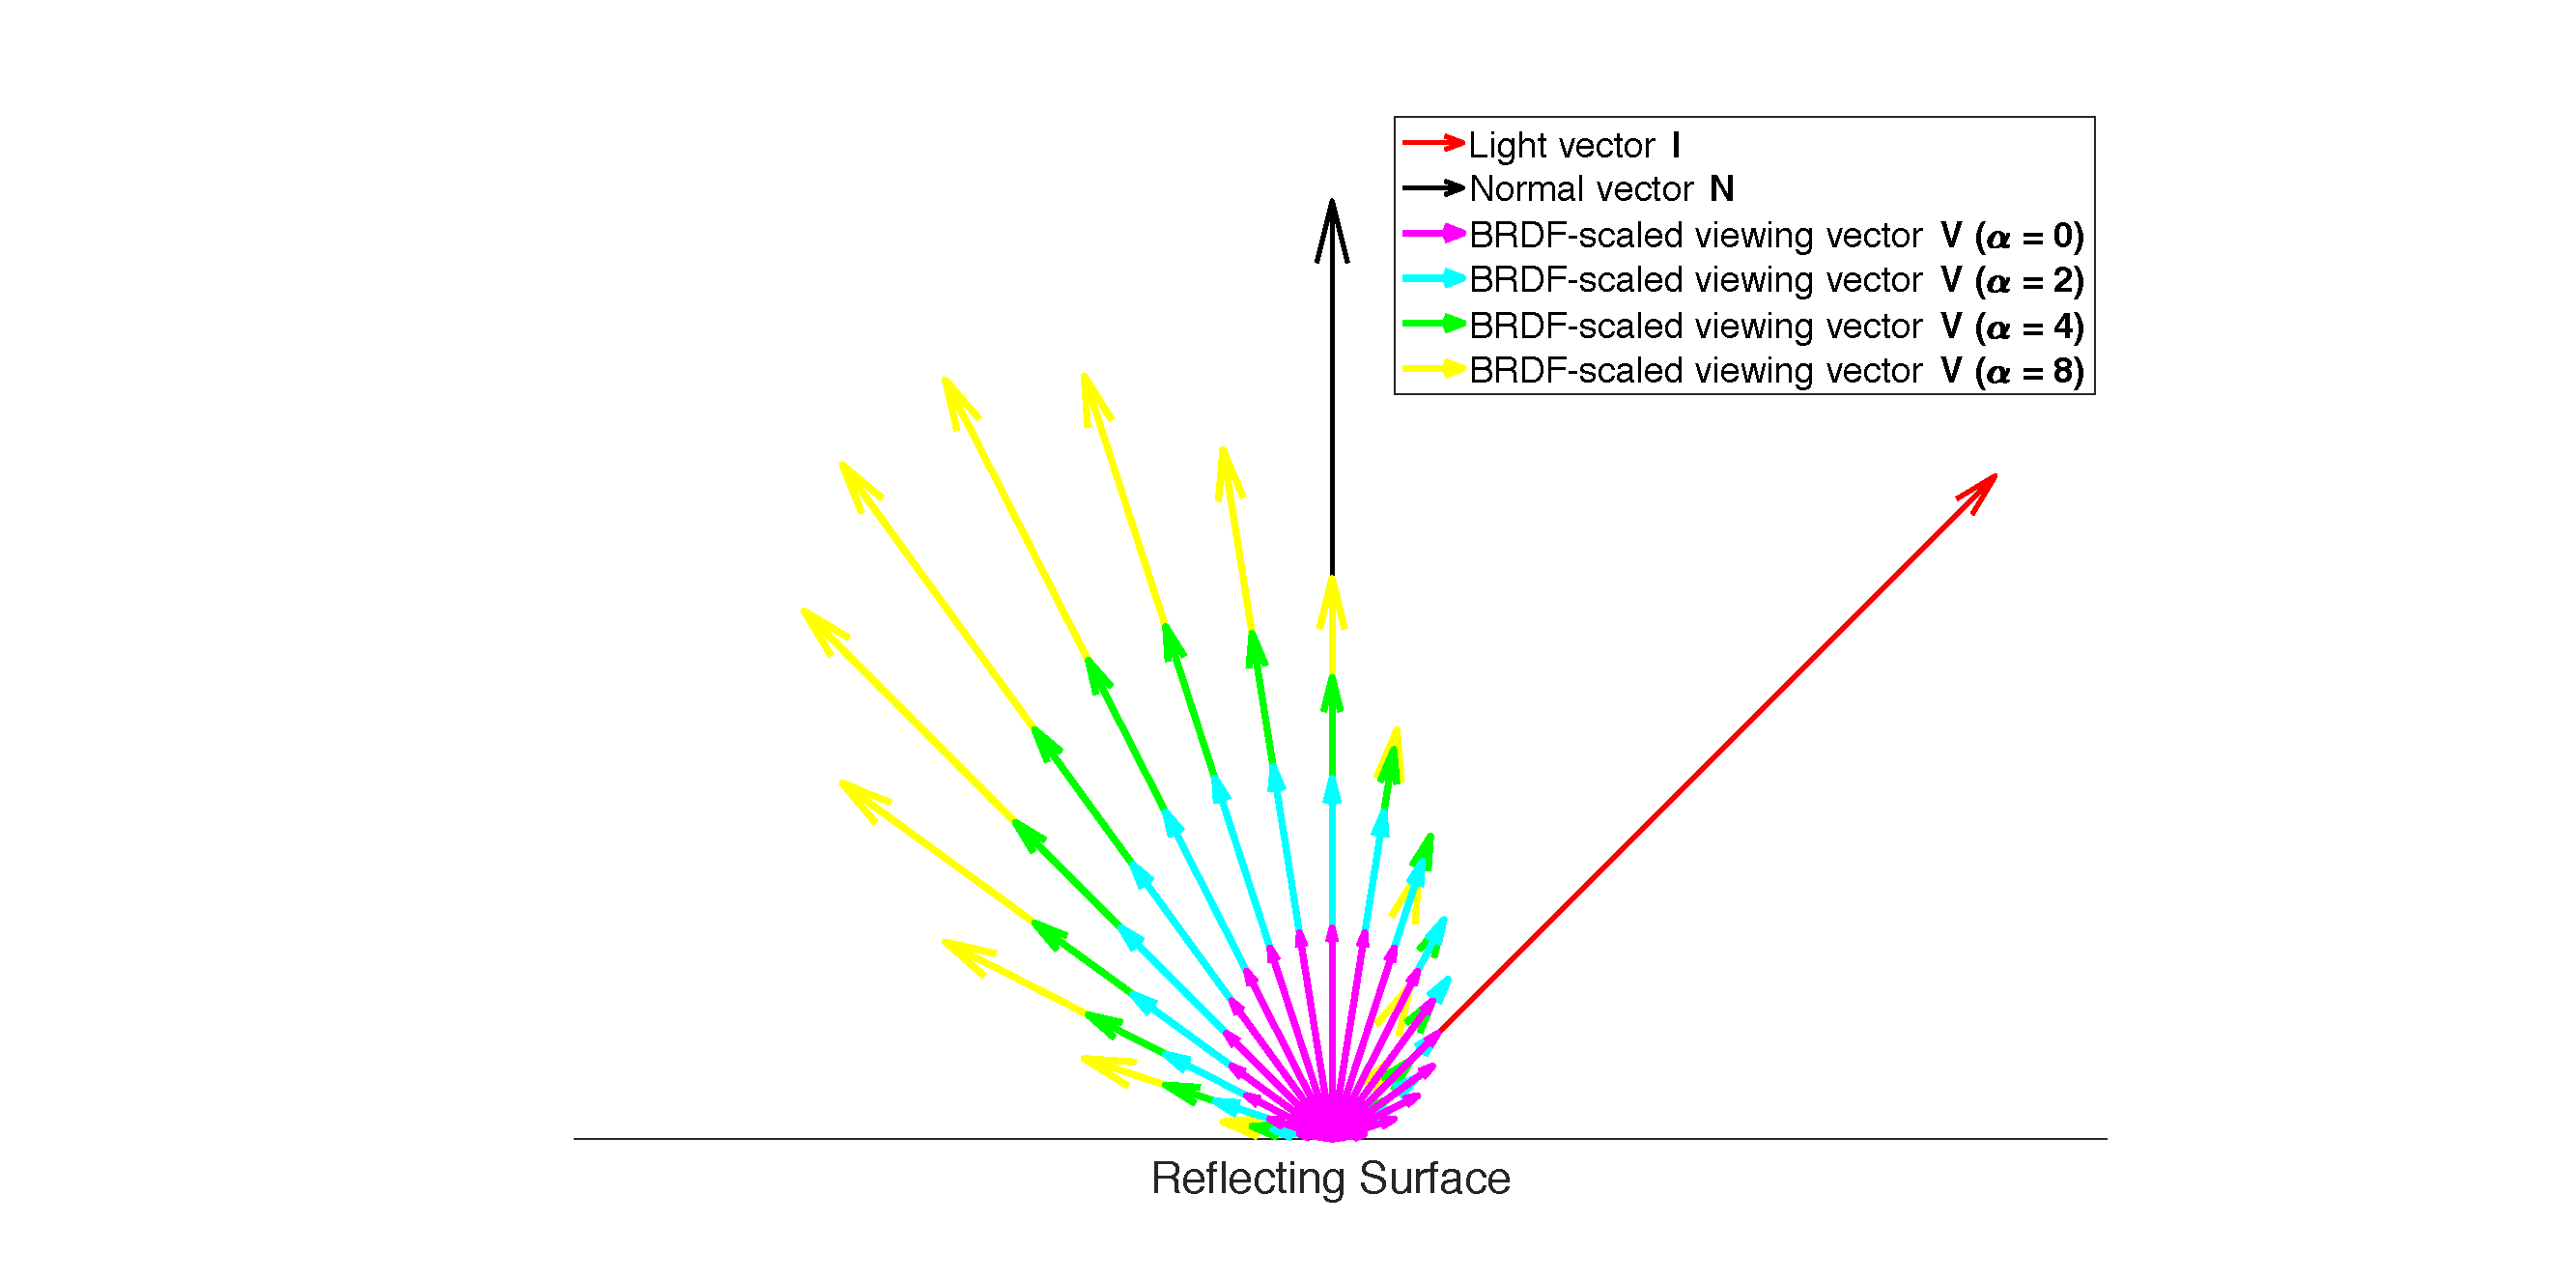
\includegraphics[width=0.8\textwidth]{./figs/BRDF_Vectors.pdf}
 \caption{Distributions of light from the Blinn--Phong model for varying values of $\alpha$, where $\mathbf{N} = (0,1)$ and $\mathbf{I} = (\cos(3\pi/4),\sin(3\pi/4))$. Again, as the value of $\alpha$ becomes large, the modeled specularity of the surface increases which results in more of the incoming light being reflected in the direction $(\cos(\pi/4),\sin(\pi/4))$.}
 \label{BRDFVectors}
\end{figure}

Optical cross section describes the maximum amount of optical flux that is reflected by an object. It can be computed accordingly by the geometry of surface of the object and reflectivity of a particular wavelength of an object. Here, we will again ignore wavelength and use the representation 
$$\sigma=\int_{S} \rho \: \mathrm{d}A$$
where $\rho$ is the optical density and is given by an $RDF$, $S$ denotes the surface. In our project, we use the representation
$$\sigma= \int_S\BRDF(\mathbf{I},\mathbf{V};\mathbf{N}) \cos\gamma\cos\beta \: \mathrm{d}A$$
with $\gamma$ denoting the relative angle between incident light angle and surface normal, $\beta$ denoting the relative angle between viewing angle and the surface normal. The cosine functions are use to account for the projected light along the surface normal. The following are some common Jacobians for projecting surfaces in parametric forms onto $\mathbb{R}^n$ (i.e. $\mathrm d A= |J| \mathrm{d}x_1...\mathrm{d}x_n)$
\begin{align}
&\nonumber\mbox{Sphere}:( r\cos\theta \sin\varphi, r\sin\theta \sin\varphi,  r\cos\varphi),   \quad |J|= r^2\sin\varphi         \\
&\nonumber\mbox{Ellipsoid} :(a\cos\theta \sin\varphi,b\sin\theta \sin\varphi,\cos\varphi),    \quad |J|=\sin\varphi  \sqrt{\sin\varphi^2( a^2\sin\theta^2+b^2\cos\theta^2)+b^2c^2\cos\varphi^2}       \\ 
&\nonumber\mbox{Cone}: (rz\cos\theta , rz\sin\theta , r),\quad |J|= rz\sqrt{1+r^2}        \\
&\nonumber\mbox{Cylinder}: ( r\cos\theta ,r\sin\theta, z), \quad |J|=r                \\
&\nonumber\mbox{Torus} :    ((c+a\cos u) \cos v,(c+a\cos u) \sin v, a\sin v), \quad |J|= a(c+a\cos v)           
\end{align}

\subsection{Rvachev Functions}~\\
The study Rvachev functions (R-functions) arises in the attempt
to describe complex geometric objects with a single inequality or equation. In the
17th century, Decartes suggested the idea of relating geometric objects (e.g.
lines, circles and bodies) to analytical objects (e.g. sets, functions and
equations). Since then, methods to study geometric properties based on its
functional descriptions have been developed systematically. This is also known
as the direct problem of analytic geometry. As oppose to the direct problem,
people also considered the inverse problem: given certain geometric objects
equipped with some desired properties, find an analytical representation to
such objects. Figure \ref{DiskAndBall} illustrates the union, intersection and difference of a disk and ball. 

\begin{figure}[H]
\includegraphics[width=.32\textwidth]{./figs/shape1.pdf}
\includegraphics[width=.32\textwidth]{./figs/shape2.pdf}
\\
\includegraphics[width=.32\textwidth]{./figs/union.pdf}
\includegraphics[width=.32\textwidth]{./figs/intersect.pdf}
\includegraphics[width=.32\textwidth]{./figs/diff.pdf}
\caption{The bottom three objects are the union, intersection, and difference of the disk and ball (top two objects).}
\label{DiskAndBall}
\end{figure}

For the simple geometric objects, the inverse problem is not
difficult. Yet for more complicated ones, especially when multiple forms
and shapes are combined, analytical descriptions become less clean and usually involve logical operations among regions defined by inequalities. The birth of R-functions is exactly to help resolve this issue.    

On the formal level, an R-function is a function whose sign do not depend on the magnitude of its arguments.  The following are some easy  examples of R-functions: 
\begin{enumerate}
\item[(a)] $f(x,y) = 1$
\item[(b)] $f(x,y,z) = x^2+y^2+z^2+1$
\item[(c)] $f(x,y) = xy$
\end{enumerate}
Here are some R-functions that are less obvious:
\begin{enumerate}
\item[(d)] $f(x,y) = \min(x,y)$
\item[(e)] $f(x,y) = x+y-\sqrt{x^2+y^2}$
\end{enumerate}
The definition of an R-function is now introduced.
\begin{definition}
A function $f(x_1,...,x_n):\mathbb{R}^n\to\mathbb{R}$ is an R-function if and only if there exists a Boolean function $F(x_1,...,x_n):\{0,1\}^n\to \{0,1\}$ such that
$$S_2(f(x_1,...,x_n))=F(S_2(x_1),...,S_2(x_n))$$
where $S_2(x)$ is defined as
$$S_2(x)=\begin{cases} 1,\quad x>0;\\ 0, \quad x<0\end{cases}$$
Such function $F$ is called the Boolean companion function of $f$.
\end{definition}

With this definition, we can easily see, for example, that (a), (c) and (d) are indeed R-functions with Boolean companions $1$, $\Leftrightarrow$ and $\wedge$
respectively. Other examples can also be checked and can have more complicated
companions. 

Upon combining elementary ``primitives" (sphere, cylinder, etc.) into composite objects with Boolean operations, we can actually construct certain R-functions that allows us to operate directly on the formulae/functions of those primitives and obtain a single analytical expression for the composite objects. And the set of R-functions used to define these operations has a natural correspondence to the Boolean functions. For the complete system of Boolean functions $\{0, \neg, \wedge, \vee\}$, consider the set of R-functions $\{-1,-x, x_1\wedge_\alpha x_2, x_1\vee_\alpha x_2\}$ where $\wedge_\alpha, \vee_\alpha$ is defined by
$$R_\alpha(x_1,x_2)=\frac{1}{1+\alpha} (x_1+x_2\pm \sqrt{x_1^2+x_2^2-2\alpha x_1x_2})$$
In the above definition, $a$ is a symmetric function in general with range $(-1,1]$. In practice, we can simply choose $a$ to be constants and the resulting R-functions are equivalent (in the same branches) in the sense that their companion Boolean functions are exactly the same, i.e. $\wedge,\vee$. There are other system of R-functions that could also be used to complete the task. For example
$$R_{\alpha}^m(x_1,x_2): \frac{1}{1+\alpha} (x_1 \wedge_\alpha ,\vee_\alpha x_2)(x_1^2+x_2^2)^{m/2}$$
One of the significant differences of $R_\alpha$ and $R_{\alpha}^{m}$ is that while $R_\alpha$ is not differentiable along the diagonal $x_1=x_2$, $R_{\alpha}^m$ is analytic on the whole plane except at $0$ where it is only $m$-times differentiable. For the purpose of this report, we shall not dwell on differentiability of the R-functions and will use $R_\alpha$. See~\cite{Shapiro} for more information.
The following example shows the merits of using R-functions. Consider defining the checkerboard in a single equation with the following constituents (primitives) 
$$D_1=\{\sin(\pi x_1)\geq 0\}, \quad D_2=\{\sin(\pi x_2)\geq 0\},\quad D_3=\{32-x^2-y^2-|x^2-y^2|\geq 0\}$$ 
Graphically, $D_1$ generates vertical stripes, $D_2$ generates horizontal stripes and $D_3$ defines region enclosed by a rectangular boundary. 
\begin{figure}[H]
\includegraphics[width=\textwidth]{./figs/checkerboard.pdf}
\end{figure}

The checker board will then be represented by the following Boolean equation
$$(D_1\vee D_2)\wedge (\bar{D}_1\vee \bar{D}_2)\wedge D_3=(D_1\Leftrightarrow D_2)\wedge D_3$$
Recall that`` $\Leftrightarrow$ " is the Boolean companion of $f(x,y)=xy$. Then the formula for checkerboard can be written as 
$(\sin(\pi x_1)\sin(\pi x_2)) \wedge_\alpha (32-x^2-y^2-|x^2-y^2|) \geq 0$
This can be further simplified into one equation with noticing that the region defined by $f(x_1,...,x_2)\geq 0$ can be written as $f-|f|= 0$.  

\subsection{OpenSCAD and Chebfun}
\subsubsection{OpenSCAD}~\\
OpenSCAD is a free software application for creating solid 3D CAD (computer-aided design) objects. It is a script-only based modeller that uses its own description language. The program does constructive solid geometry (CSG) using specified geometric primitives (such as spheres, boxes, cylinders, etc.) and defines how they are modified and combined (for instance by intersection, difference, envelope combination and Minkowski sums) to render a more complex 3D model. Then we use other tool (Gmsh, etc.) to create finite element meshes. Figure \ref{fig:sdh_openscad} demonstrate the example of screwdriver handle constructed by OpenSCAD and the triangular mesh generated on the surface of the object.
\begin{figure}[H]   	
\centerline{\includegraphics[scale=0.3]{./figs/sdh_openscad}
     	\hspace{-6pt}
		\includegraphics[scale=0.2]{./figs/sdh_mesh}}
     	\hspace{-6pt}
		\caption{Constructive Solid Geometry \& Generation of Finite element mesh ~\cite{mesh}}
        \label{fig:sdh_openscad}
\end{figure}

Numerically, we can handle even more complex objects through the typical procedure. However, to accurately represent the surface many thousands to millions of facets are sometimes required and a trade-off must be made between accuracy of the surface represented and speed of calculation. Table \ref{table: sphere OCS} shows the numerical calculation of OCS for a unit sphere. The relative error is about $10^{-4}$ by using 20480 triangle facets.  

We wish to develop a method that improves the accuracy for much more complex objects. We consider representing the surface in functional form using Chebyshev polynomials and built up through Rvachev functions. The reason to choose Chebyshev polynomial is because for smooth enough object surface, by using sufficiently many Chebyshev poins, the surface representation is possibly accurate to close to machine precision.

\subsubsection{Chebyshev interpolation analysis}~\\
It's common to choose the base points $x_i$ for interpolation to be evenly spaced. In many cases, the data to be interpolated are available only in some certain forms, for instance, when the data consist of instrument readings separated by a constant time interval. Meanwhile, in other cases, for example, the sine function - we are free to choose the base points as we see the better fit. It turns out that the choice of base point spacing can have a significant efffect on the interpolation error. Chebyshev interpolation refers to a particular optimal way of spacing the points.

Consider the case with single variable. We start with a function $y=f(x)$ and take data points from it to build an interpolating polynomial $P(x)$. The interpolation error evaluated at $x^*$ is $f(x^*)-P(x^*)$. The following theorem gives a formula for the interpolation error that is usually impossible to evaluate exactly, but often can be at least bounded by an error.
\begin{theorem}
Assume that $P(x)$ is the (degree $n-1$ or less) interpolating polynomial fitting the $n$ pionts $(x_1,y_1),...,(x_n,y_n)$. The interpolation error is 
\begin{equation} \label{eqn_poly_error}
f(x)-P(x)=\frac{(x-x_1)(x-x_2)\cdot\cdot\cdot(x-x_n)}{n!}f^{(n)}(c)
\end{equation}
where $c$ lies between the smallest and largest of the number $x,x_1,...,x_n.$
\end{theorem}
The motivation for Chebyshev interpolation is to improve control of the maximum value of the interpolation error given by ~\eqref{eqn_poly_error}. For a given positive integer $n$, the Chebyshev nodes in the interval $(-1,1)$ are
\begin{equation}
\label{eqn_cheb_point}
x_i=\cos\Big(\frac{2i-1}{2n}\pi\Big),\mbox{ }i=1,...,n.
\end{equation}
The interpolation error due to Chebyshev positioning formula ~\eqref{eqn_cheb_point}, is summarized in the following theorem:
\begin{theorem}
The choice of real numbers $-1\le x_1,...,x_n\le 1$ that makes the value of 
\begin{equation}
\max_{-1 \leq x \leq 1}|(x-x_1)\cdot\cdot\cdot(x-x_n)|
\end{equation}
as small as possible is given by ~\eqref{eqn_cheb_point}, and the minimum value is $\dfrac{1}{2^{n-1}}$. In fact, the minimum is achieved by 
\begin{equation} \label{eqn_cheb_error}
(x-x_1)\cdot\cdot\cdot(x-x_n)=\frac{1}{2^{n-1}}T_n(x)
\end{equation}
where $T_n(x)$ denotes the degrees $n$ Chebyshev polynomial.
\end{theorem}

\begin{exmp}
In this example, we compare the errors for Polynomial interpolation and Chebyshev interpolation with different interpolation points for the function $e^x$ on $[-1,1]$. FIGURE \ref{fig:e1} shows the comparisons for $N=5$ and $N=8$, and there isn't significant difference between the two interpolations for $N=5$. In the contrast, we can see better approximation for the Chebyshev interpolation near the boundary when  $N=8$.\\
The interpolation formula ~\eqref{eqn_poly_error} gives 
\begin{equation}
f(x)-P_4(x)=\frac{(x+1)(x+\frac{1}{2})x(x-\frac{1}{2})(x-1)}{5!}f^{(5)}(c)
\end{equation}
where $-1<c<1$. For $-1\leq x\leq 1$, the error is bounded by
\begin{equation*}
f(x)-P_4(x)=\frac{(x+1)(x+\frac{1}{2})x(x-\frac{1}{2})(x-1)}{5!}f^{(5)}(c)\leq \frac{0.11348}{5!}e\approx 0.002570
\end{equation*}
The interpolation formula ~\eqref{eqn_cheb_error} gives 
\begin{equation*}
|e^x-P_4(x)|\leq \frac{e}{2^45!}\approx 0.00142
\end{equation*}

\begin{figure}[H]     	\centerline{\includegraphics[width=3.2in]{./figs/e1a.eps}
      	\hspace{-6pt}
     	\includegraphics[width=3.2in]{./figs/e1b.eps}}
     	\hspace{-6pt}
		\caption{Errors of interpolations for the fucntion $e^x$ with points $N=4$ and $N=8$}
        \label{fig:e1}
\end{figure}
\end{exmp}

\begin{exmp}
In this example, we interpolate function $f(x)=1/(1+12x^2)$ by using both polynomial and Chebyshev method with 15 points. Figure \ref{fig:e2} shows Runge phenomenon from polynomial interpolation.
\begin{figure}[H] 	
        \centerline{\includegraphics[width=3.2in]{./figs/e2a.eps}
      	\hspace{-6pt}
     	\includegraphics[width=3.2in]{./figs/e2b.eps}}
     	\hspace{-6pt}
		\caption{Interpolation of function $f(x)=\frac{1}{1+12x^2}$}
        \label{fig:e2}
\end{figure}
\end{exmp}

\section{Results and Discussions}
\subsection{Analytical Solutions for Sphere}$~\\$
Recall that by using Blinn--Phong model for sphere, we can compute OCS through
$$\sigma =\iint_{A}\BRDF(\mathbf{I},\mathbf{V};\mathbf{N}) \cos\gamma \cos\beta \mathbf{\chi}_{\ip{N}{I}\geq 0}\mathbf{\chi}_{\ip{V}{N}\geq 0} \: dA$$
where $\gamma$ is the angle between $\mathbf{N}=(\cos\vartheta\sin\varphi,\sin\vartheta\sin\varphi,\cos\varphi)$ and  $\mathbf{V}=(V_1, V_2, V_3)$,  $\beta$ is the angle between $\mathbf{N}$ and $\mathbf{I}=(I_1,I_2,I_3)$. The geometric relations are shown in the picture below.

\begin{figure}[h!]
  \includegraphics[width=4in]{./figs/Sphere_edit.pdf}
  \label{fig:sphere}
\end{figure}
The appearances of two indicator functions 
$$\mathbf{\chi}_{\ip{N}{I}\geq 0}=\{(\vartheta,\varphi):\cos\vartheta\sin\varphi I_1+\sin\vartheta\sin\varphi I_2+\cos\varphi I_3\geq 0\}$$ 
$$\mathbf{\chi}_{\ip{V}{N}\geq 0}=\{(\vartheta,\varphi): \cos\vartheta\sin\varphi V_1+\sin\vartheta\sin\varphi V_2+\cos\varphi V_3\geq 0\}$$ 
in the formula are just to include only the common part of the illuminated area and the detectable area.
The spherical coordinates $(r,\vartheta,\varphi)$ are related to the Cartesian coordinates $(x,y,z)$ via
$$x =r\cos\vartheta \sin\varphi, \quad y=r\sin\vartheta \sin\varphi, \quad z=r\cos\varphi $$
with Jacobian 
$$\bigg|\frac{\partial(x,y,z)}{\partial(r,\vartheta,\varphi)}\bigg|= r^2 \sin\varphi $$
Thus by noticing 
$$\cos\gamma =\frac{\ip{\mathbf{N}}{\mathbf{V}}}{\|\mathbf{N}\| \|\mathbf{V}\|},\quad \cos\beta=\frac{\ip{\mathbf{N}}{\mathbf{I}}}{\|\mathbf{N}\| \|\mathbf{I}\|}$$
we arrive at
  $$\sigma =\int_{0}^{2\pi}\int_{\frac{\pi}{2}}^{-\frac{\pi}{2}}\Bigg(\frac{\ip{\mathbf{I}+\mathbf{N}}{\mathbf{V}}}{\|\mathbf{I}+\mathbf{N}\|}\Bigg)^\alpha\frac{\ip{\mathbf{N}}{\mathbf{V}}}{\|\mathbf{N}\| \|\mathbf{V}\|}\frac{\ip{\mathbf{N}}{\mathbf{I}}}{\|\mathbf{N}\| \|\mathbf{I}\|}r^2\sin\varphi\mathbf{\chi}_{\ip{\mathbf{N}}{\mathbf{V}}\geq 0}\mathbf{\chi}_{\ip{\mathbf{N}}{\mathbf{I}}\geq 0} \: d\vartheta \: d\varphi$$
  
\subsection{Numerical Calculation of Scattering Function for Sphere - Finite Element Approach}~\\
For each facet in the model, find angle $\theta$ between incident ray and facet normal, in FIGURE \ref{fig:facet}. Target relativity, $\rho$, is given by $MRDF$($\theta$), and scattering function, $\sigma$, is estimated by
\begin{equation}
\sigma =\frac{\rho A}{\Omega}
\end{equation} 
where $A$ is target area, $\Omega$ is solid angle of scattering.

Simply for a sphere, we generate a mesh by using icosahedron. An icosahedron is a polyhedron composed of twenty identical equilateral, each triangle has the same area and each vertex is at the same distance from all its neighbors. To get a higher number of triangles we need to subdivide each triangles by creating a new vertex at the middle point of each edge which is then normalized, to make it lie in the sphere surface. This breaks the initial properties of the icosahedron, the triangles are not equilateral anymore and neither the area nor the distance between adjacent vertices is the same across the mesh. But it is still a better approximation by almost any measure excluding its number of triangles. 

\begin{figure}[H]  	\centerline{\includegraphics[height=1.4in,width=1.2in]{./figs/facet.png}}
		\caption{Incident angle $\theta$ on each triangle facet}
        \label{fig:facet}
\end{figure}

\begin{figure}[H] 	\centerline{\includegraphics[width=4.8in]{./figs/icosahedron.eps}}
		\caption{Visualization of icosahedral mesh with number of faces N = 20, 80, 320, 1280, 5120 and 20480}
        \label{fig:icosahedron}
\end{figure}

The calculation of optical cross section is summarized as following:
\begin{itemize}
\item Genete mesh for a given model
\item For each facet, calculate reflectance from incident angle, material properties, etc.
\item Sum over all visible facets to obtain OCS
\end{itemize} 
The following Table \ref{table: sphere OCS} shows the numerical results for different mesh size of a sphere with constant $\rho=1$ and $\alpha=0$. The analytical OCS for a sphere is $2\pi/3\approx 2.094395102389723$.
\begin{table}[H]
	\small
	\caption{Numerical calculation of OCS for a sphere
	}
	\centering
	\begin{tabular}{|c|c|c|c|c|c|}
	\hline
	N & Numerical Results & Relative error & order \\
	\hline
	320 & $1.99294$ & $4.84419-02$ &  \\
    \hline	
	1280 & $2.06845$ & $1.23853E-02$ & 0.98381 \\
    \hline	
	5120 & $2.08787$ & $3.11387E-03$ & 0.99593 \\
	\hline
	20480 & $2.09276$ & $7.79570E-04$ & 0.99898 \\
	\hline
	\end{tabular}
	\label{table: sphere OCS}
\end{table}
  
\subsection{Numerical Solutions for Sphere \& Application to Ellipsoid}

To capture the target area for numerical integration using Chebfun, the boolean relationship is incorporated to avoid defining explicit boundary angles. This is achieved by multiplying the integrand derived from the Blinn--Phong model by $\max\{0, \langle \mathbf{L},\mathbf{N}\rangle\}$ and $\max\{0,\langle \mathbf{V},\mathbf{N}\rangle\}$ which rules out area not in the intersection of the lighted area and viewer's range. Here $\langle\cdot, \cdot\rangle$ is the inner product, $\mathbf{L}$ is the light source direction, $\mathbf{V}$ is the viewer direction, and $\mathbf{N}$ is the outward unit normal of the surface.

{\bf Case 1: Method verification.} Verification of the accuracy of Chebfun is performed by simulating the case where the light source and the viewer are at the identical direction to capture the optical cross section value. The reflexivity and the light diffusivity of the surface are fixed as $\rho = 1$ and $\alpha =0$ respectively. The optical cross section (OCS) approximated using Chebfun, with interpolating error tolerance of $10^{-8}$, yields $\sigma_{cheb} = 2.094395102389723$. The known analytical solution is $\sigma_{analytical} = 2\pi/3 \approx 2.094395102393195$. The absolute error of the Chebfun approach is in the range of $10^{-12}$ due its semi-analytical nature. This is superior to the triangular discretization approach which performs at $\approx 10^{-4}$ accuracy. To ensure the Chebfun approach does not produce non-physical result, additional tests were run for different $\alpha$ value and different viewer's position.

\begin{figure}[h]
\centering 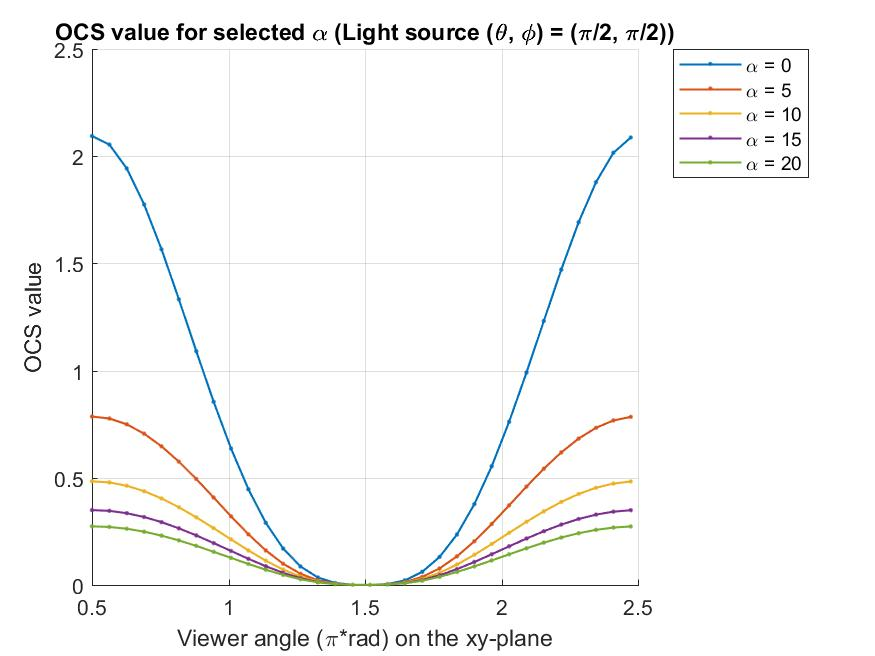
\includegraphics[scale=0.4]{./figs/OCS_parallel_plane}    
\caption{Simulation of orbiting viewer on the plane as the light source with different $\alpha$ values.}    
\label{OCSParallelPlane}
\end{figure}

\begin{figure}[h]
\centering 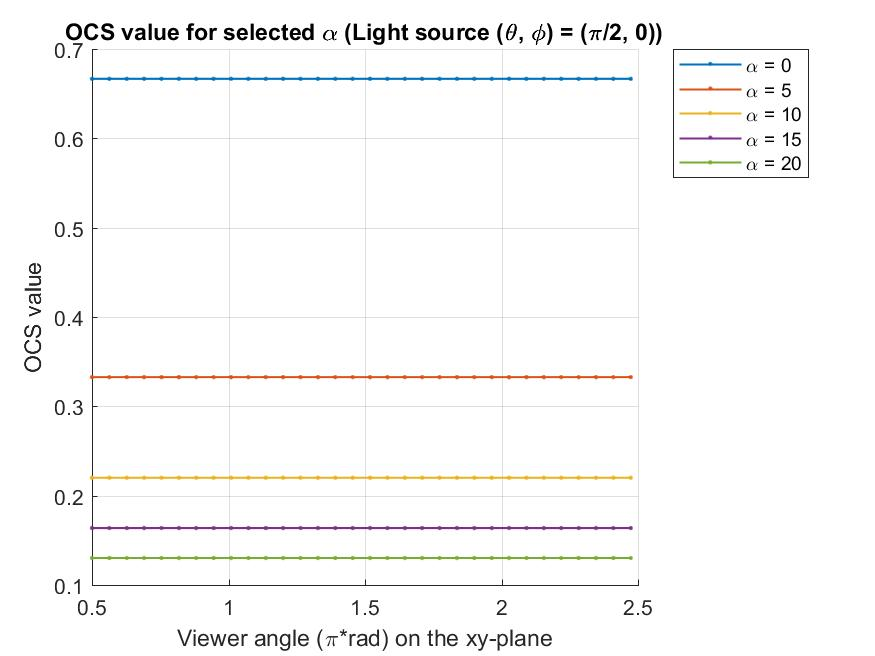
\includegraphics[scale=0.4]{./figs/OCS_perpendicular_plane}
\caption{Simulation of orbiting viewer on the plane perpendicular to the light source with different $\alpha$ values.}
\label{OCSPerpendicularPlane}
\end{figure}

The $\alpha$ value is chosen to be the interval $[0,18]$ with fixed increment. The results shows that as $\alpha$ increases the OCS value decreases (Figure \ref{OCSParallelPlane}). Since higher $\alpha$ value represents the smaller specular highlight, the viewer would receive less total reflected light across the whole surface. This is in agreement with the physical observation.

Next we tested the influence of the viewer position. Two scenarios were tested: parallel orbiting viewer and perpendicular orbiting viewer, with respect to the light source. In the parallel orbiting scenario (Figure \ref{OCSParallelPlane}), the OCS value decreases as the viewer moves away from the light source, followed by restoration to the initial value. The rate of decay is clearly influenced by the $\alpha$ value. In the perpendicular orbiting scenario, the viewer moves on the xy-plane while the light source is fixed at $(\theta, \phi) = (0,0)$ position. The simulation results shows that the OCS value remains constant.

Both orbiting simulation results show agreement with the physical phenomenon. This indicates that Chebfun approach can produce accurate and physical results.

\begin{figure}[h]
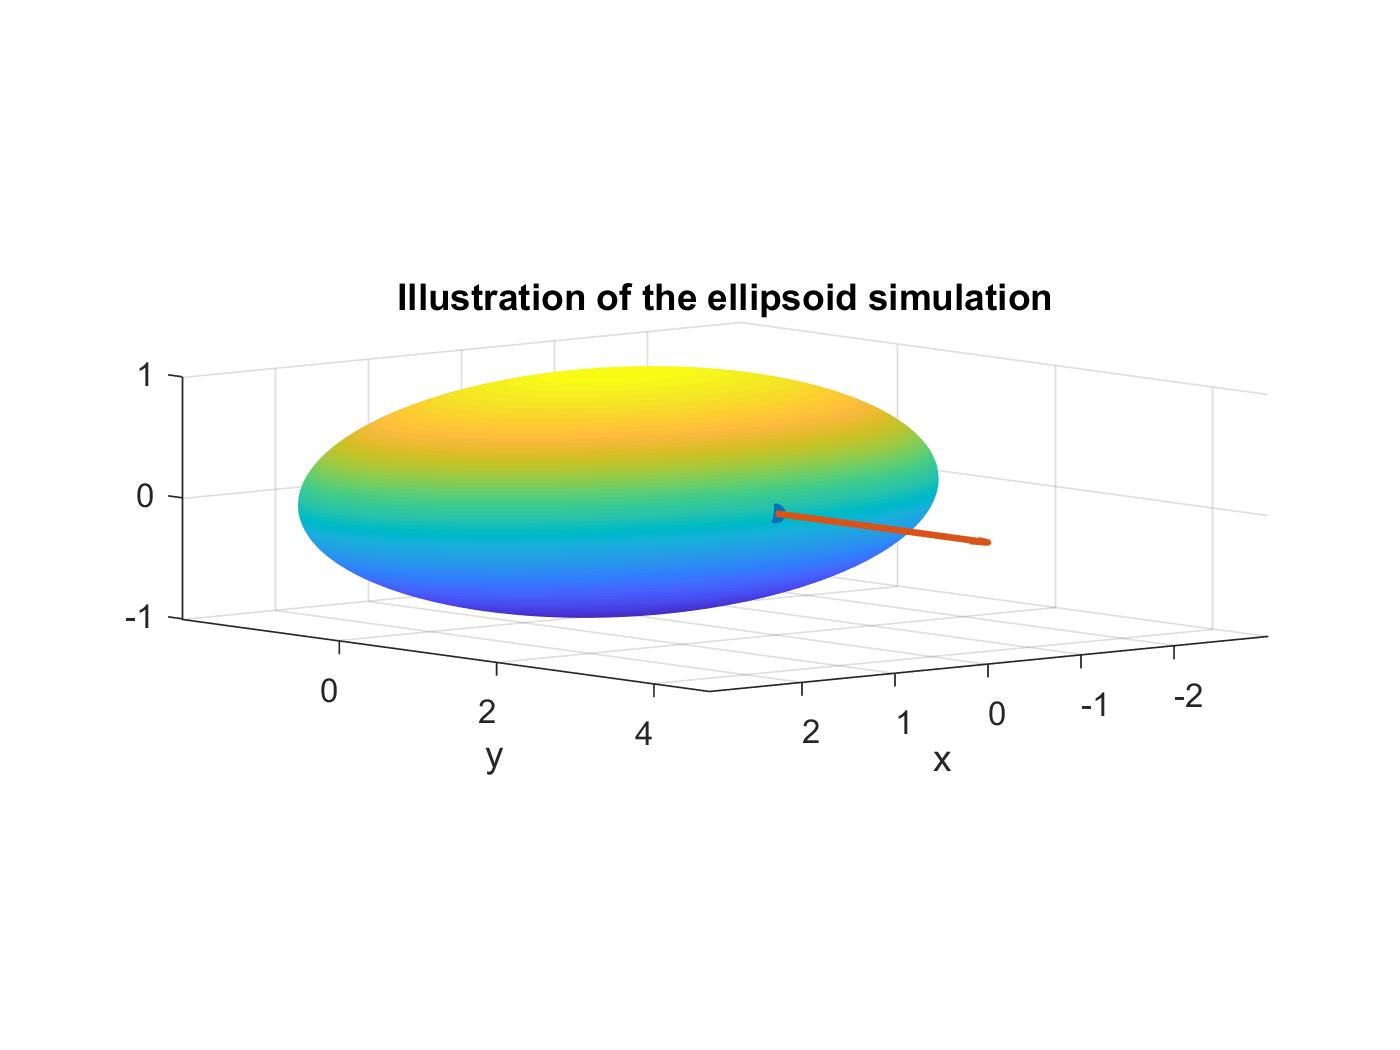
\includegraphics[scale=0.35]{./figs/OCS_ellipsoid}
\caption{A visual representation of the ellipsoid I simulation. The red line represents the direction of the incoming light source. It can be observed that how fast the curvature change when the viewer orbits around the ellipsoid. The graphic is generated using the Chebfun package.}
\label{OCSEllipsoid}
\end{figure}

\begin{figure}[h]
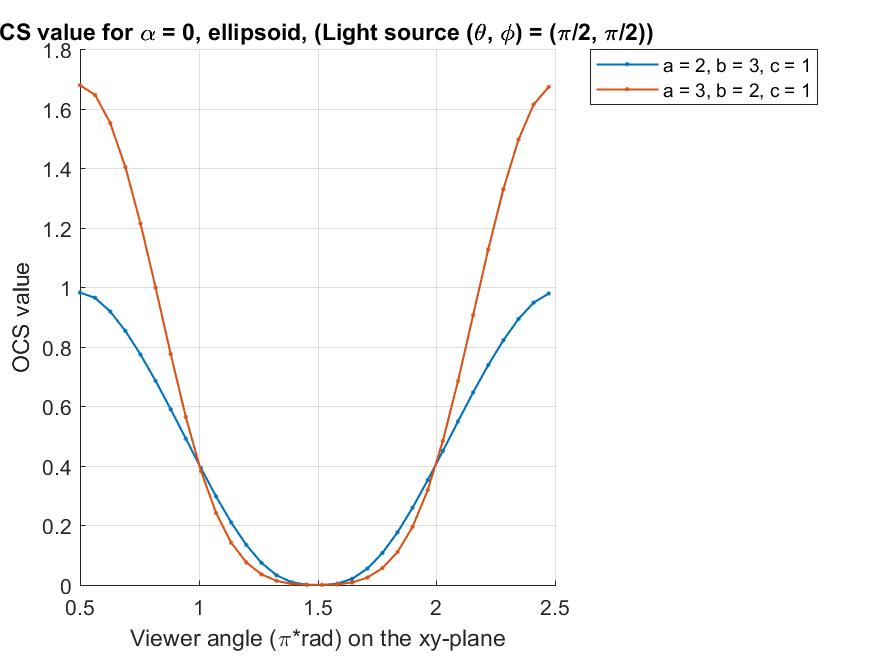
\includegraphics[scale=0.35]{./figs/OCS_parallel_plane_ellipsoid}
\caption{Simulation of orbiting viewer on the same plane as the light source. $\alpha = 0$. The shape of interest here is an ellipsoid.}
\label{OCSParallelPlaneEllipsoid}
\end{figure}

{\bf Case 2: Ellipsoid I} Following the verification we applied the Chebfun approach to a non-uniform shape. The shape chosen is an triaxial ellipsoid due to its simple geometry and non-uniform symmetry. We started with the ellipsoid $\frac{x^2}{4}+\frac{y^2}{9}+\frac{z^2}{1} = 1$. $\rho$ and $\alpha$ are as in the verification section. However, due to the artificial singularities generated from the parameterization of the surface, we intentionally excluded a small neighborhood near the ``north pole" and the``south pole" to avoid instability. Light source is fixed at $(\theta,\phi) = (\pi/2, \pi/2)$ and the viewer orbits on the $xy$-plane. The Chebfun approach yields OCS value $\approx 0.9821$ when the viewer and the light source are at the identical direction. This lower observed value is likely due to the difference in curvatures of the surface facing $(\theta, \phi)=(\pi/2, \pi/2)$ comparing to a hemisphere. While in the sphere case, the angle between the unit normal and the viewer direction increases at a constant rate, in the ellipsoid case the the angle approaches 90 degree at a faster rate. Similar to the sphere case, the OCS value drops down as the viewer moves further away from the light source. The decay rates of OCS value between the sphere and ellipsoid case are expected to be different and can be observed using Figure \ref{OCSParallelPlane} and Figure \ref{OCSParallelPlaneEllipsoid}. We also performed the same test simulating viewer orbiting on a plane perpendicular to the light source, the resulting periodic oscillation obtained is determined to be physical.

{\bf Case 3: Ellipsoid II} We next chose the ellipsoid described by $\frac{x^2}{9}+\frac{y^2}{4}+\frac{z^2}{1} = 1$ to compare the result with ellipsoid I case. The remaining setup is identical to the previous case. Using the Chebfun approach we found that the OCS value when the light source and the viewer are at the identical position is about 1.6786. Since the viewer would be facing a larger area, the OCS value is expected to be higher. The result turns out to be as expected such that the OCS value produced is higher than the previous case. Finally we looked at the decay rate of the OCS value based on the increase of specular highlight. The result indicates that even though the geometry has noticeable influence on how fast the OCS decreases, but at the long run the decay rate would likely converge to the same value.

\begin{figure}[h]
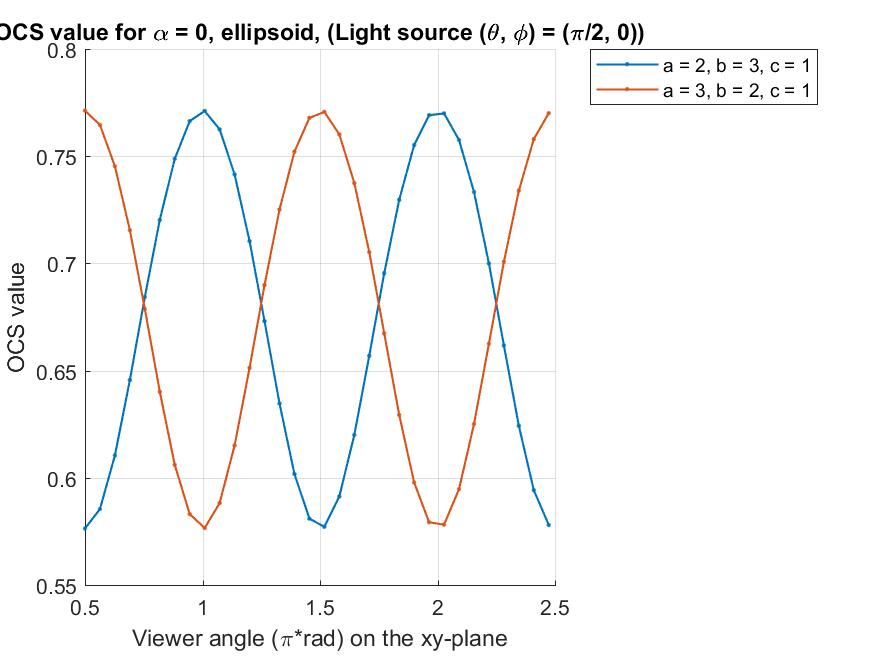
\includegraphics[scale=0.23]{./figs/OCS_perpendicular_plane_ellipsoid}
\caption{Simulation of orbiting viewer on the plane perpendicular to the light source. $\alpha = 0$. The shape of interest here is an ellipsoid.}
\label{OCSPerpendicularPlaneEllipsoid}
\end{figure}

\begin{figure}[h]
\includegraphics[scale=0.2]{./figs/OCS_decay_by_alpha_ellipsoid}
\caption{OCS value of the ellipsoid simulations with increasing $\alpha$ values. It can be observed that ellipsoid I experiences a faster decay due to the high curvature decay.}
\label{OCSDecaybyAlphaEllipsoid}
\end{figure}

\section{Future work}
\subsection{Other Shapes and Technical Challenges}$~\\$
\textbf{\indent Creating complex shapes and visualization.}
Using Rvachev functions, it is possible to create 
complex objects by combining basic shapes such as elliptic paraboloids, 
planes, and spheres. In Figure~\ref{fig:rocket}, we show a model rocket created
using this approach. Finding the correct sequence of shapes and Rvachev
functions, is in general non-trivial. Another issue is finding 
an appropriate visualization tool. For this purpose, 
we used the MATLAB code \verb+ezimplot3+ which can be 
found in MATLAB Central~\cite{Morales}.

\begin{figure} 
\centerline{\includegraphics[width=.7\textwidth]{rocket.pdf}} 
\caption{A model rocket created by combining basic shapes via Rvachev
functions.}
\label{fig:rocket} 
\end{figure} 

\textbf{Numerical approximation issues.}
In the pursuit of accurate solutions of optical cross section for more complex
objects, one major challenge arises when the object being considered has sharp
edges. Even in one dimension, polynomial approximation can be challenging for
functions that are not differentiable everywhere, such as $f(x) = |x|$ on the
interval $[-1,1]$. Even with R-functions providing a means of obtaining
implicit representations for combinations of objects, these implicit
representations often contain terms that make polynomial approximation
difficult. For example, the implicit function obtained using R-functions that
describes the union of two spheres of radius one with centers at the origin and
$(1.5,0,0)$ is
\[{\left(x-\frac{3}{2}\right)}^2-\sqrt{{\left(x^2+y^2+z^2-1\right)}^2+{\left({\left(x-\frac{3}{2}\right)}^2+y^2+z^2-1\right)}^2}+x^2+2\,y^2+2\,z^2-2 = 0
\]
One solution could be to manually increase the tolerance (and thus decrease the
desired accuracy) of the polynomial approximation, though doing so for complex
objects might yield approximations that are far less accurate that using facets
to discretize the surface. Another approach might be to use smoothed versions
of objects, such as the equation $x^n + y^n + z^n = 1$ for large even values of
$n$ to approximate a cube centered at the origin (see Figure \ref{cubes}).
While there will certainly be a trade-off in the accuracy, investigation will
be needed to fully evaluate the viability of this approach and to compare it
with the approach of simply increasing the approximation tolerance.

\begin{figure}[H]
\includegraphics[width=\linewidth]{./figs/cubes.pdf}
\caption{An example of approximating an object with sharp edges. Here a cube is approximated by the function $x^n + y^n + z^n = 1$ for $n = 2$, 4, and 8 (from left to right).}
\label{cubes}
\end{figure}

\subsection{The Multipath Problem}~\\
Let's now consider the case where light projected on a concave surface. Unlike the previous cases, the light detected by the sensor can be reflected multiple times from points on the surface other points on the surface due to concavity. Theoretically, the bouncing of light can go on infinitely if there is no energy dissipation. The surface we consider here is the half cylindrical shell facing downwards and the radius of the cylinder is $r$. Given $\psi_I$, we denote the incident light by its vector of direction $\mathbf{I}_1=(\cos\psi_I,\sin\psi_I)$ and the light detector has viewing angle $\mathbf{V}$. For lights that are reflected by the surface at $D_1,D_2,...,D_n$ before it is collected by the light detector, denote the (inward) normal vector at $D_n$ by $\mathbf{N}_n=(-\cos\vartheta_n,-\sin\vartheta_n)$ and unit vector for $\overrightarrow{D_{n}D_{n-1}}$ by $\mathbf{I}_n=(-\cos\psi_n,-\sin\psi_n)$.  Define inductively 
$$(*)\begin{cases}\mathbf{I}_1=\mathbf{I}=(\cos\psi_{I},\sin\psi_{I}),\\ \delta_n=\vartheta_{n+1}-\vartheta_n,\\ \psi_n=\psi_{n-1}-(\pi-\delta_n)\end{cases}$$ 

\begin{proposition}
Consider the situation described above. The Optical Cross Section under such circumstances is computed as
$$\sigma=\sum_{n}^{\infty}\sigma_n$$
with
\begin{multline*}
\sigma_n =\int_{0}^{\pi}...\int_{0}^{\pi}\Bigg(\frac{\ip{\mathbf{I}_n+\mathbf{N}_n}{\mathbf{V}}}{\|\mathbf{I}_n+\mathbf{N}_n\|}\Bigg)^\alpha\frac{\ip{\mathbf{N}_n}{\mathbf{V}}}{\|\mathbf{N}_n\| \|\mathbf{V}\|}\frac{\ip{\mathbf{N}_n}{\mathbf{I}_n}}{\|\mathbf{N}_n\| \|\mathbf{I}_n\|} \\\prod_{i=1}^{n-1}\bigg\{ \Bigg(\frac{\ip{\mathbf{I}_i+\mathbf{N}_i}{\mathbf{V}}}{\|\mathbf{I}_i+\mathbf{N}_i\|}\Bigg)^\alpha \frac{\ip{\mathbf{N}_i}{\mathbf{V}}}{\|\mathbf{N}_i\| \|\mathbf{V}\|}\frac{\ip{\mathbf{N}_i}{\mathbf{I}_i}}{\|\mathbf{N}_i\| \|\mathbf{I}_i\|}\frac{1}{\|rN_{i+1}-rN_i\|^2}\bigg\}r^n\: \mathrm{d}\vartheta_1...\mathrm{d}\vartheta_n\end{multline*}
assuming that the infinite sum and the integral both converge.
\end{proposition}

\begin{proof}
The proof is very straightforward. The contribution from a single bounce to the OCS is easily computed by using Bling-Phong's model with the projected $\BRDF$
$$\sigma_1 =\int_{0}^{\pi}\Bigg(\frac{\ip{\mathbf{I}_1+\mathbf{N}_1}{\mathbf{V}}}{\|\mathbf{I}_1+\mathbf{N}_1\|}\Bigg)^\alpha\frac{\ip{\mathbf{N}_1}{\mathbf{V}}}{\|\mathbf{N}_1\| \|\mathbf{V}\|}\frac{\ip{\mathbf{N}_1}{\mathbf{I}_1}}{\|\mathbf{N}_1\| \|\mathbf{I}_1\|} r\:\mathrm{d}\vartheta_1$$
To compute the contribution from lights that bounce multiple times before it is received, what we need is just to write the relations between the angles correctly. For the case with two bounces, we can deduce these relations with the help from the picture below. Observe that now
$\angle{ID_1O}=\angle{OD_1D_2}=\angle{D_1D_2O}$ and $\vartheta_1=\vartheta_2+\angle{D_2D_1O}+\angle{OD_1I}$. Hence by defining $\delta_2=\vartheta_2-\vartheta_1$, $\angle{D_2D_1O}+\angle{OD_1I}=\pi-\delta_2$. So the polar angle $\psi_2$ for $\mathbf{I}_2$ can be written as $\psi_1-(\pi-\delta_2)$.  More generally,  the relations among the angles for even more bounces are given by  $(*)$.
\begin{figure}[H]
  \includegraphics[width=4in]{./figs/multipath_edit.pdf}
  \label{fig:reflection}
\end{figure}

Now let's compute the contribution for lights that bounce exactly $n$ times (happening at $D_1,...,D_n$ respectively) before they are received. For each bounce happening at $D_i$, a differential length around $D_1$ becomes the new emitter that shines towards another differential length around $D_{i+1}$. The viewing angle from $D_{i+1}$ towards $D_i$ now is just the direction of the reflected light $\mathbf{I}_{i}$. So we can invoke Blinn-Phong model to compute the detectable light at $D_{i+1}$ from $D_i$ and get the projected $\BRDF$
$$\BRDF^*_{D_i}=\Bigg(\frac{\ip{\mathbf{I}_i+\mathbf{N}_i}{\mathbf{I}_{i+1}}}{\|\mathbf{I}_i+\mathbf{N}_i\|}\Bigg)^\alpha\frac{\ip{\mathbf{I}_i}{\mathbf{N}_i}}{\|\mathbf{I}_i\|\|\mathbf{N}_i\|}\frac{\ip{\mathbf{I}_{i+1}}{\mathbf{N}_i}}{\|\mathbf{I}_{i+1}\|\|\mathbf{N}_i\|} \frac{1}{\|r\mathbf{N}_{i+1}-r\mathbf{N}_i\|^2}$$
Therefore, for the lights that bounce exactly $n-$times before reaching the detector, their total contributions to $OCS$ would be 
\begin{equation*}
\sigma_n =\int_{0}^{\pi}...\int_{0}^{\pi}\Bigg(\frac{\ip{\mathbf{I}_n+\mathbf{N}_n}{\mathbf{V}}}{\|\mathbf{I}_n+\mathbf{N}_n\|}\Bigg)^\alpha\frac{\ip{\mathbf{N}_n}{\mathbf{V}}}{\|\mathbf{N}_n\| \|\mathbf{V}\|}\frac{\ip{\mathbf{N}_n}{\mathbf{I}_n}}{\|\mathbf{N}_n\| \|\mathbf{I}_n\|} \bigg(\prod_{i=1}^{n-1}\BRDF^*_{D_i}\bigg) r^n\: \mathrm{d}\vartheta_1...\mathrm{d}\vartheta_n
\end{equation*}

The appearance of factor $r^n$ is due to the Jacobians from rewriting line integrals into usual integrals. Total contributions for up to $n$ bounces is then given by
 $$ \sigma= \sigma_1+\sigma_2+...+\sigma_n$$
 \end{proof}
 
\section{Conclusion}

In this work we have investigated several aspects of the light reflection. Our main goals were to understand the diffusivity of the reflection associated with material of the surface. To do so first we construct and de-construct complex geometric shapes using Rvachev function which is based on boolean operations. Rvachev functions help obtaining functional representation of the surface that does not require storage of information such as vertices, unit normal vectors and triangle adjacency.
Second, we improve the current discrete model to continuous model favoring less data storage and we learned to use the combination of Chebfun and indicator function, a computation tool that takes the advantage of Chebyshev polynomial interpolation to perform numerical integration over the surface with less need of explicit expression.
Finally, we extend the continuous model to incorporate the multi-path phenomenon starting from simple case of two-dimensional one reflection model and extended the result to build the theory for three-dimensional n reflections model.

\section{Acknowledgment}

\begin{thebibliography}{9}
\bibitem{BRDF}
Chris Wynn,
\emph{An Introduction to BRDF-Based Lighting}.
NVIDIA Corporation, 2000.

\bibitem{Ward}
Gregory J. Ward, 
\emph{Measuring and Modeling Anisotropic Reflection. (SIGGRAPH 92),}: 265-272 (1992).

\bibitem{BlinnPhong}
James F. Blinn,  
\emph{Models of light reflection for computer synthesized pictures}, Proc. 4th
Annual Conference on Computer Graphics and Interactive Techniques: 192-198
(1977). 

\bibitem{CookTorr}
Robert Cook and Kenneth Torrance,
\emph{A reflectance model for computer graphics. Computer Graphics}, Proc. of SIGGRAPH 81: 244-253 (1981).  

\bibitem{Shapiro}
Vadim Shapiro,
\emph{Theory of R-functions and Applications: A Primer}, Cornell University, 1988.

 \bibitem{Boolean Operations}
Yohan D. Fougerolle, Andrei Gribok, Sebti Foufou, Frederic Truchetet and Mongi A. Abidi,
\emph{Boolean Operations with Implicit and Parametric Representation of Primitives Using R-Functions}.
IEEE Transactions on Visualization and Computer Graphics, Vol. 11, No. 5 (2005).

\bibitem{CSG Operations}
Younis Hijazi, Aaron Knoll, Mathias Schott, Andrew Kensler, Charles Hansen and Hans Hagen,
\emph{CSG Operations of Arbitrary Primitives with Interval Arithmetic and Real-Time Ray Casting}.
Scientific Visualization: Advanced Concepts, 78-89 (1998) 
	
 
\bibitem{Zachary}
  Zachary Battles and Lloyd N. Trefethen,
  \emph{An Extension of Matlab to Continuous Function and Operations}.
  SIAM J. SCI. COMPUT Vol. 25, No. 5: 1743-1770 
 
\bibitem{mesh}
\url{http://sfepy.org/doc-devel/preprocessing.html}

\bibitem{Morales}
Gustavo Morales. Matlab Central.\\
\url{https://www.mathworks.com/matlabcentral/fileexchange/23623-ezimplot3-implicit-3d-functions-plotter?focused=5168229&tab=function}


	



\end{thebibliography}

\bibliographystyle{plain}
%\bibliography{paper}

\end{document}
